\documentclass[journal=gmj]{report}%
%%%% Packages
\usepackage{graphicx}
\usepackage{multicol,multirow}
\usepackage{amsmath,amssymb,amsfonts}
\usepackage{mathrsfs}
\usepackage{amsthm}
\usepackage{rotating}
\usepackage{appendix}
\usepackage{ifpdf}
\usepackage[T1]{fontenc}
\usepackage{newtxtext}
\usepackage{newtxmath}
\usepackage{textcomp}
\usepackage{xcolor}
\usepackage{lipsum}
\usepackage{xeCJK}
\usepackage{fontspec}
\usepackage{subcaption}
\usepackage{float}
% 设置字体路径和字体文件
\setmainfont[
    Path=../assets/font/,    % 字体所在路径
    Extension=.ttc,          % 字体文件扩展名
    UprightFont=Songti,      % 字体名称(在 ttc 文件中找到具体名称)
]{Songti}

\usepackage[colorlinks,allcolors=blue]{hyperref}

\newtheorem{theorem}{Theorem}[section]
\newtheorem{lemma}[theorem]{Lemma}
\newtheorem{remark}[theorem]{Remark}

% 定义样式为定义型
\theoremstyle{definition}
\newtheorem{definition}[theorem]{Definition}
\newtheorem{example}[theorem]{Example}

% 公式按章节编号
\numberwithin{equation}{section}


\jname{GA deception}
\articletype{Research Report}
\jyear{2024}


\begin{document}

\begin{Frontmatter}
\center
    
\title[Article Title]{遗传算法欺骗问题}

% There is no need to include ORCID IDs in your .pdf; this information is captured by the submission portal when a manuscript is submitted. 
\author{专业: 数学与应用数学\quad 学号: 3210101613\quad 姓名: 罗俊勋}

\keywords{genetic algorithm, deception, optimization}

\abstract{遗传算法(GA)是一种基于自然选择和遗传学原理的优化方法,广泛应用于解决复杂的优化问题。然而,遗传算法在某些特定条件下可能遭遇“欺骗问题”,即算法可能会错误地被引导到局部最优解,导致无法有效寻找全局最优解。本文深入探讨了遗传算法中的欺骗问题,并以最小欺骗问题(MDP)为例,分析了欺骗现象的产生机制。进一步,我们提出了引入无义密码子、动态变异率和多点变异等改进策略,以提高算法的多样性和鲁棒性,并通过实验验证了这些方法在不同问题场景中的有效性。}

\end{Frontmatter}

\section*{引言}

遗传算法(Genetic Algorithm, GA)是一种模拟自然选择和遗传机制的优化算法,广泛应用于求解复杂的优化问题。然而,在实际应用中,遗传算法常常遇到一个严重的挑战——欺骗问题。该问题发生在某些特定环境下,其中局部最优解邻域的平均适应度高于全局最优解邻域的平均适应度,从而导致遗传算法错误地引导搜索过程,偏离全局最优解。这种现象使得算法容易陷入局部最优解,进而无法有效进行全局搜索。

欺骗问题的产生与遗传算法的基本机制密切相关。根据模式定理,遗传算法的本质是对不同模式进行搜索。如果最优解所在模式的平均适应度低于次优解所在模式的平均适应度,就很容易导致欺骗问题的发生。

在本文中,我们将以最小欺骗问题(MDP)为例,分析欺骗问题产生的原因,并提出一系列优化方法,旨在尽可能减少欺骗问题的影响。

\localtableofcontents

\section{欺骗性}

\subsection{基本概念}

\begin{definition}[模式(Scheme)]
   一个字符串,由染色体字母表中的字母和通配符组成。模式是一个集合,例如在二进制编码中 $H = 0*1* = \{0010, 0011, 0110, 0111\}$。
\end{definition}

\begin{definition}[模式阶(Schema Order)]
    模式 $H$ 中确定基因位的个数,记为 $O(H)$,例如 $O(001*0*) = 4$。
\end{definition}

\begin{definition}[模式定义长度(Schema Defining Length)]
    模式 $H$ 中第一个确定位置和最后一个确定位置之间的距离称为模式的定义长度,记作 $\delta(H)$,例如 $\delta(0*1*0**) = 4$。
\end{definition}

\begin{definition}[竞争模式]
    若在模式 $H$ 和 $H^\prime$ 中,$*$ 的位置完全一致,但任一确定位的编码均不相同,则称 $H$ 和 $H^\prime$ 为竞争模式。
\end{definition}

\subsection{定义}

\begin{definition}[欺骗性]
    设 $f(X)$ 的最大值对应的 $X$ 集合为 $X^*$,$H$ 为包含 $X^*$ 的 $m$ 阶模式,$H$ 的竞争模式为 $H^\prime$,且满足 $f(H) > f(H^\prime)$,则称 $f$ 为 $m$ 阶欺骗。

    其中,
    $$
    f(H) = \frac{1}{|H|}\sum\limits_{X\in H} f(X)
    $$

    $|H|$ 为模式 $H$ 中的个体数。
\end{definition}

\section{最小欺骗问题(MDP)}

\subsection{两类欺骗问题}

在 1987 年,Goldberg \cite{goldberg1987deceptive} 提出了一个最小欺骗问题(Minimal Deceptive Problem, MDP),该问题是一个二进制编码的最大化问题。假设有以下标记和模式及其适应度:

$$
\begin{array}{c}
    (11):\, **1****1*, \, f_{11} \\
    (00):\, **0****0*, \, f_{00} \\
    (10):\, **1****0*, \, f_{10} \\
    (01):\, **0****1*, \, f_{01}
\end{array}
$$

假设 $f_{11}$ 为全局最优解,即:

$$
f_{11} > f_{00}, f_{10}, f_{01}
$$

若假设 $f(0*) > f(1*)$,则可得到两种类型的欺骗问题:

$$
\begin{cases}
  \text{Type I} & f_{01} > f_{00}\\
  \text{Type II} & f_{00} > f_{01}
\end{cases}
$$

Goldberg 指出,对于遗传算法(GA)而言,$\text{Type II}$ 比 $\text{Type I}$ 更难解决,因此我们将重点关注第二类欺骗问题($\text{Type II}$)。

\subsection{Goldberg 欺骗实例}

以下是 Goldberg 给出的 $\text{Type II}$ 欺骗问题的一个例子:

$$
f_{11} = 1.1 ;\quad f_{00} = 1.0 ;\quad f_{01} = 0.9 ;\quad f_{10} = 0.5
$$

当次优解 $(00)$ 的初始比例较大时,它会替代最优解。下面的图示展示了不同初始比例($p_{00}$)对算法性能的影响:

\begin{figure}[H]
    \centering
    % 第一行
    \begin{subfigure}[b]{0.45\textwidth}
        \centering
        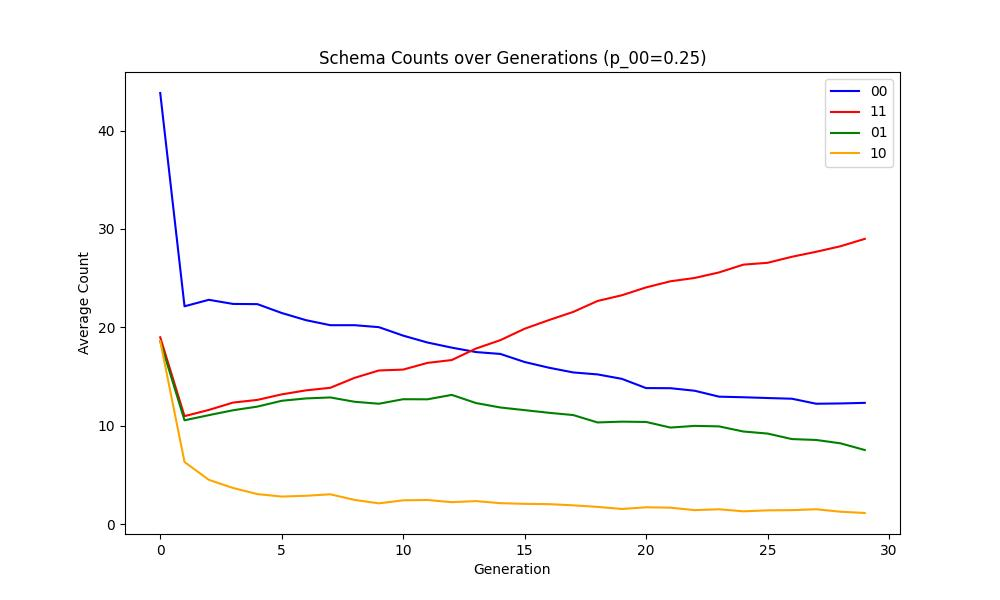
\includegraphics[width=\textwidth]{../assets/img/popnum_with_p00_0.25}
        \caption{\( p_{00} = 0.25 \)}
    \end{subfigure}
    \hfill
    \begin{subfigure}[b]{0.45\textwidth}
        \centering
        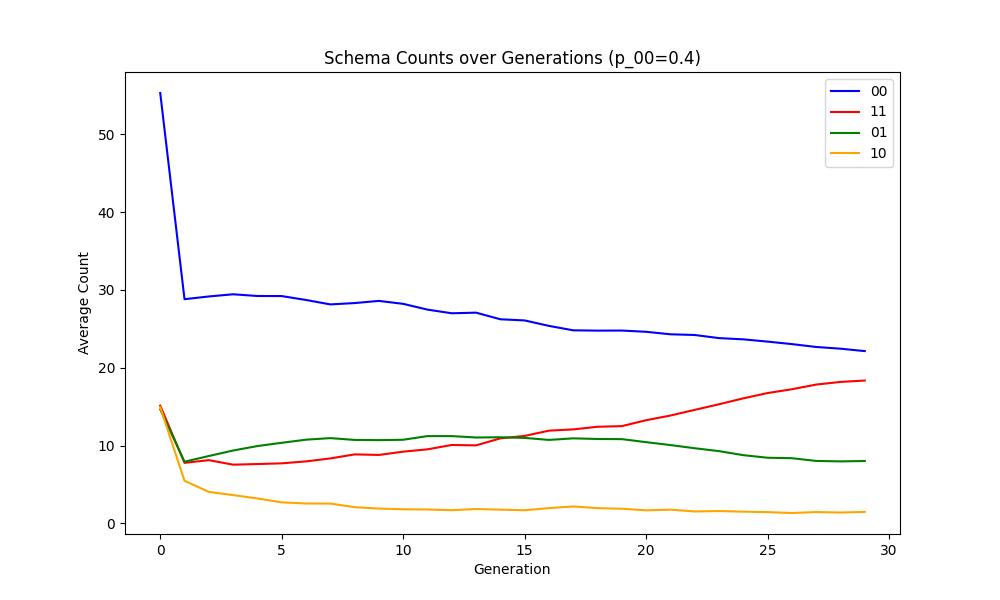
\includegraphics[width=\textwidth]{../assets/img/popnum_with_p00_0.4}
        \caption{\( p_{00} = 0.40 \)}
    \end{subfigure}
    
    % 第二行
    \begin{subfigure}[b]{0.45\textwidth}
        \centering
        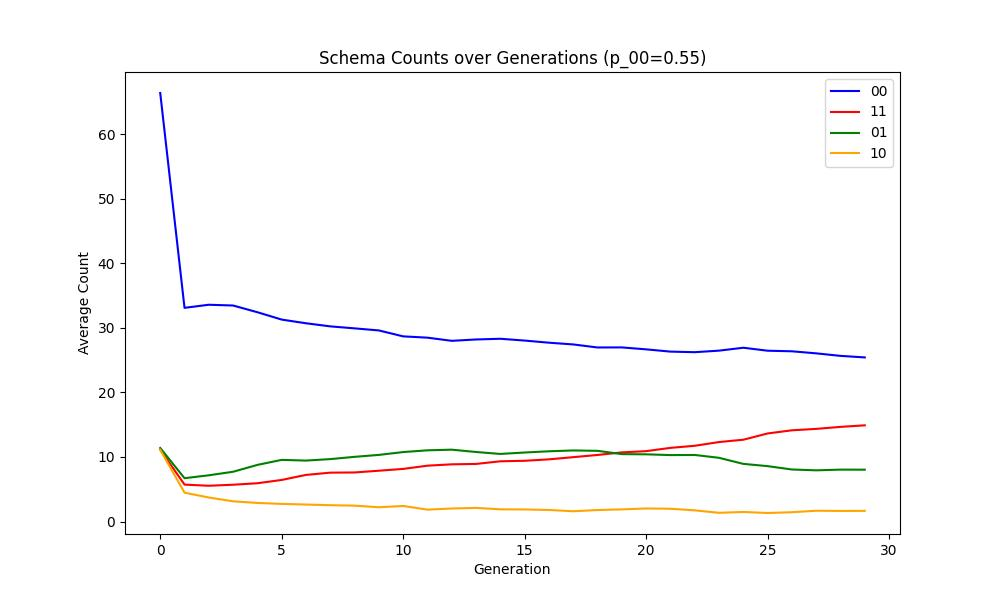
\includegraphics[width=\textwidth]{../assets/img/popnum_with_p00_0.55}
        \caption{\( p_{00} = 0.55 \)}
    \end{subfigure}
    \hfill
    \begin{subfigure}[b]{0.45\textwidth}
        \centering
        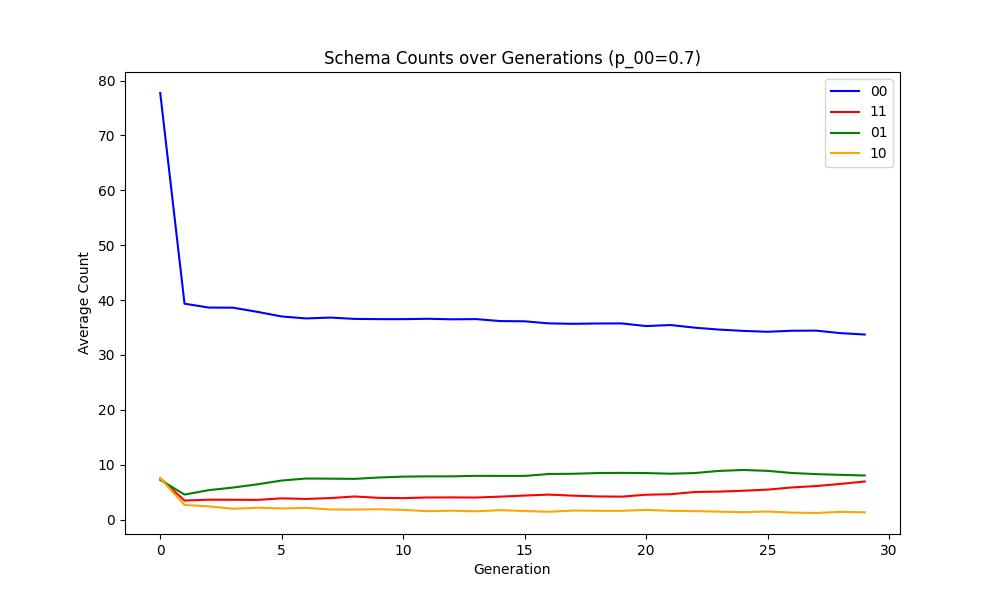
\includegraphics[width=\textwidth]{../assets/img/popnum_with_p00_0.7}
        \caption{\( p_{00} = 0.7 \)}
    \end{subfigure}
    
    \caption{不同 \( p_{00} \) 下的模式计数对比。}
    \label{fig:schema_counts}
\end{figure}

这一结果表明,对于 $\text{Type II}$ 欺骗问题,初始比例对算法的性能有显著影响。这个问题尤为棘手,因为大多数情况下我们无法提前“知道”最优解的位置,尤其是在高维问题中。因此,当函数在定义域的绝大部分区域都表现为欺骗性时,算法的性能会显著下降。

同样地,在选择交叉率和变异率时也存在类似的问题。对于一个具体的求解问题,我们通常不知道“最佳的参数组合”是什么,因此不希望算法的效果过于依赖于这些参数的选择。

\section{无义密码子}

\subsection{原理及其应用}

为了解决遗传算法中初始参数选择的问题,我们可以借鉴自然遗传学中的无义密码子的概念,以此来增加种群多样性并增强算法的鲁棒性 \cite{NOVKOVIC1998895}。

\begin{definition}[无义密码子]
    在生物学中,无义密码子 \cite{baikeWuYi} 是指那些不编码任何氨基酸的密码子,也被称为终止密码子。例如,在 DNA 中,UAG、UAA 和 UGA 都是无义密码子。

    在蛋白质合成过程中,由于这些密码子缺乏相应的反密码子 tRNA,蛋白质合成因此无法继续,从而发挥了终止蛋白质合成的重要作用。
\end{definition}

无义密码子在蛋白质合成中的作用 \cite{proteinSynthesis} 是:核糖体沿着 mRNA 读取密码子,当遇到无义密码子时,蛋白质合成会终止,导致蛋白质链的提前截断。这种终止机制会影响蛋白质的长度和结构,从而改变其功能。

类似地,在遗传算法(GA)中,我们可以引入“无义密码子”机制,作为一种附加信息来影响染色体的交叉和变异等过程。这一设计能够有效增加染色体的多样性,避免算法陷入局部最优解,并提高算法的鲁棒性。

为了实现无义密码子的功能,我们需要在遗传算法的基本流程中引入相应的机制。具体而言,在生成初始种群时,为每个染色体引入一个交叉概率和变异概率。在后续的迭代过程中,交叉和变异将基于每个染色体上携带的概率,而不是固定的概率。

引入遗传废料的遗传算法(GAW, Genetic Algorithm with Waste)在理论上可以完全消除算法对初始参数设置的依赖性。这种方法的特点如下:
\begin{itemize}
    \item \textbf{初始参数独立性}:遗传废料确保参数的随机分布,从而降低对初始参数设置的依赖。
    \item \textbf{增强鲁棒性}:遗传废料有助于缓解种群早熟收敛问题,尤其是在适应度景观复杂的情况下。
    \item \textbf{搜索空间探索能力}:在不依赖种群收敛的优化问题中,GAW 是一种有效的搜索工具,能够大幅提升全局解的探索能力。
\end{itemize}

传统的自适应参数设置方法(如基于适应度值的动态调整)通过适应度函数来决定参数变化,而遗传废料的参数变化则独立于适应度。这种独立性使得 GAW 在解决未知问题时具有更高的鲁棒性和灵活性。

\subsection{实验验证}

我们优化的目标函数为:

$$
f(x) = \sin(x) + \cos(5x) + \frac{1}{1 + 0.4x^2} + 3, \quad x \in D = [-10, 10]
$$

\begin{figure}[H]
    \centering
    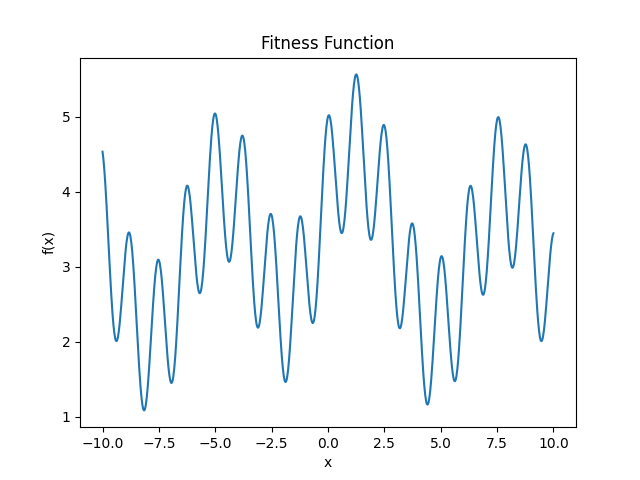
\includegraphics[width=0.45\textwidth]{../assets/img/fitness_function.png}
    \caption{目标函数的适应度值。}
    \label{fig:fitness}
\end{figure}

\subsubsection{设计思路}

\begin{itemize}
  \item \textbf{编码方式:} 长度为 $k$ 的向量,元素取值在定义域 $D$ 中,其中 $k$ 为染色体长度。
  \item \textbf{适应度计算:} 取染色体元素适应度值的平均值。
  \item \textbf{交叉算子:} 单点交叉。
  \item \textbf{变异算子:} 随机选择一个基因位点,并将其变异为一个随机数。
  \item \textbf{选择算子:} 轮盘赌选择。
  \item \textbf{设定参数:} $p_m = 0.1$,$p_c = 0.9$。
  \item \textbf{GW 参数设定:} 在染色体的最后两个位置添加两个浮点数,作为交叉和变异的概率,其中 $p_{m_{gw}} = \text{np.random.uniform}(0, 0.2)$,$p_{c_{gw}} = \text{np.random.uniform}(0.8, 1)$。
    \begin{itemize}
      \item \textbf{带 GW 的交叉概率:} 两个染色体的交叉概率取两个染色体的交叉概率的平均值。
      \item \textbf{带 GW 的变异概率:} 两个染色体的变异概率取两个染色体的变异概率的平均值。
    \end{itemize}
\end{itemize}

\subsubsection{实验结果}

\begin{figure}[H]
  \begin{center}
    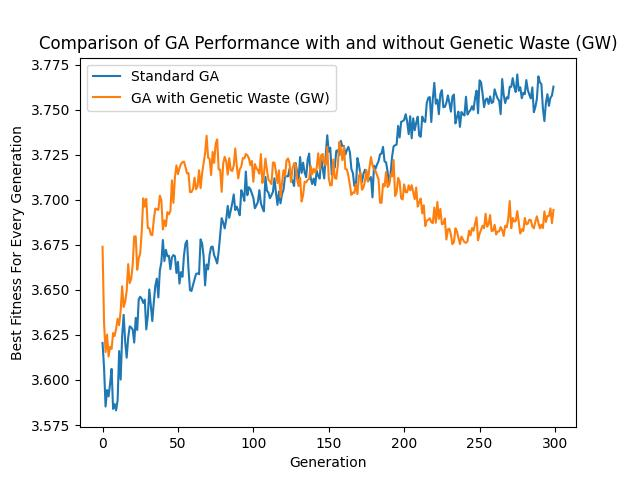
\includegraphics[width=0.45\textwidth]{../assets/img/comparison_gw_vs_standard.jpg}
  \end{center}
  \caption{GAW 与 GA 的比较。}
  \label{fig:comparison}
\end{figure}

\subsection{结论}

在算法运行的初期,带有 GW 的算法种群多样性较高,能够更有效地探索解空间。然而,在算法后期,由于 GW 的引入,收敛速度较慢。

GW 通过提供可变的变异率来增加种群的多样性,尤其是在算法初期,这种多样性帮助算法探索更广泛的解空间。然而,随着算法的进行,变异操作的影响需要逐渐减弱,以维持种群的均匀性并加速收敛。否则,过高的变异率可能会导致种群难以收敛,进而影响算法的性能。

为了解决这一问题,可以结合缩放函数逐步减小变异率的影响,从而减少潜在的破坏性变异。通过引入这种“阻尼”函数,能够在算法的后期更好地控制变异操作,促进算法向最优解收敛。在需要种群收敛的优化问题中,缩放函数的使用对于保持算法的稳定性和加速收敛速度至关重要。


\section{动态变异率}

\subsection{原理及其应用}

动态变异率是一种根据算法运行状态自动调整变异率的方法。其基本思想是在算法的不同阶段使用不同的变异率,以平衡探索(exploration)和开发(exploitation)的需求。在算法的初期阶段,较高的变异率有助于探索更广泛的解空间,避免陷入局部最优解;而在算法的后期阶段,较低的变异率有助于细化搜索,促进算法向全局最优解的收敛。

\subsection{常见方法}

\paragraph{线性递减法}

在此方法中,变异率随着代数的增加而线性递减,公式为:

$$
p_{m_{\text{gen}}} = p_{m_{\text{max}}} - \frac{p_{m_{\text{max}}} - p_{m_{\text{min}}}}{\text{maxgen}} \times \text{gen}
$$

其中,$p_{m_{\text{gen}}}$ 是当前代的变异率,$p_{m_{\text{max}}}$ 是初始变异率,$p_{m_{\text{min}}}$ 是最小变异率,$\text{maxgen}$ 为最大代数,$\text{gen}$ 是当前代数。

\paragraph{指数递减法}

该方法通过指数衰减函数使变异率逐渐减小,公式为:

$$
p_{m_{\text{gen}}} = p_{m_{\text{max}}} e^{-\lambda \frac{\text{gen}}{\text{maxgen}}}
$$

其中,$\lambda$ 是衰减速率,用于控制变异率递减的速度。

\subsection{与 GW 的结合}

在 GW 算法中,我们可以将指数递减法应用于变异率的调整。具体的变异率变化公式为:

$$
p_{m_{\text{gw},\text{gen}}} = p_{m_{\text{gw}}} e^{-\lambda \frac{\text{gen}}{\text{maxgen}}}
$$

该公式中,$p_{m_{\text{gw},\text{gen}}}$ 是带有 GW 机制的变异率,$\lambda$ 控制递减速率,$\text{gen}$ 和 $\text{maxgen}$ 分别表示当前代数和最大代数。

\subsection{实验验证}

\begin{figure}[H]
  \centering
  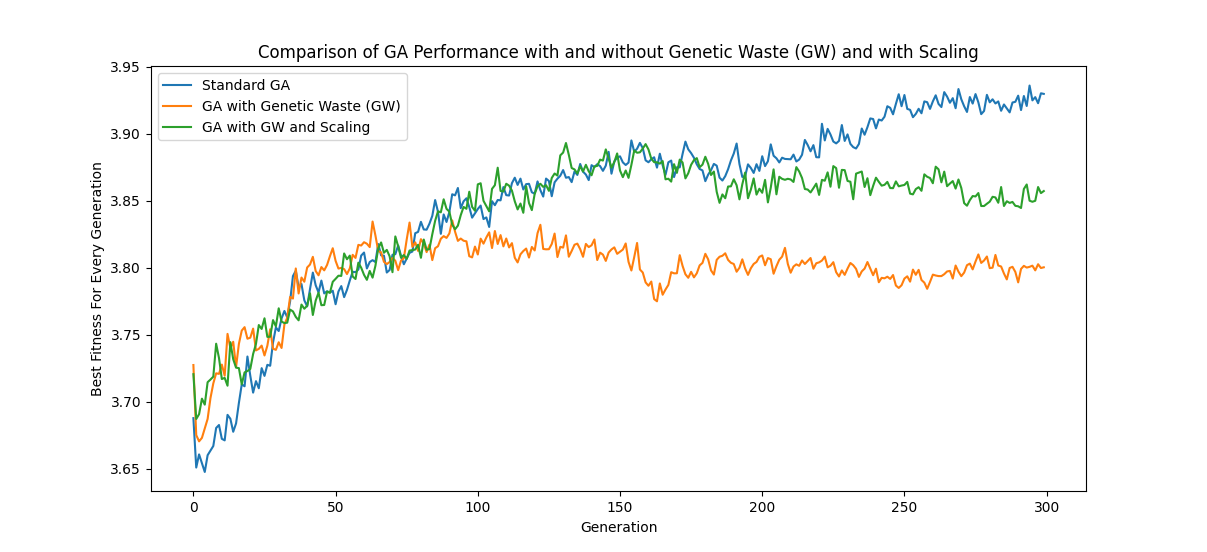
\includegraphics[width=0.95\textwidth]{../assets/img/comparison_gw_vs_standard_vs_gwscaling.png}
  \caption{GA 与 GAW、带缩放因子的 GAW 的比较}\label{fig:}
\end{figure}

\subsection{结论}

从实验结果可以看出,引入动态变异率的 GW 算法在算法的后期阶段能够更快地收敛到全局最优解,显著提高了算法的性能。

\section{多点变异}

\subsection{原理及其应用}

多点变异是一种在变异操作中引入多个变异点的策略。其基本思想是,通过引入多个变异点,可以增加种群的多样性,提升算法的全局搜索能力。在传统的单点变异中,只有一个基因位点会发生变异,而在多点变异中,多个基因位点可以同时变异,从而更有效地增加种群的多样性。

\subsection{实验验证}

\begin{figure}[H]
  \centering
  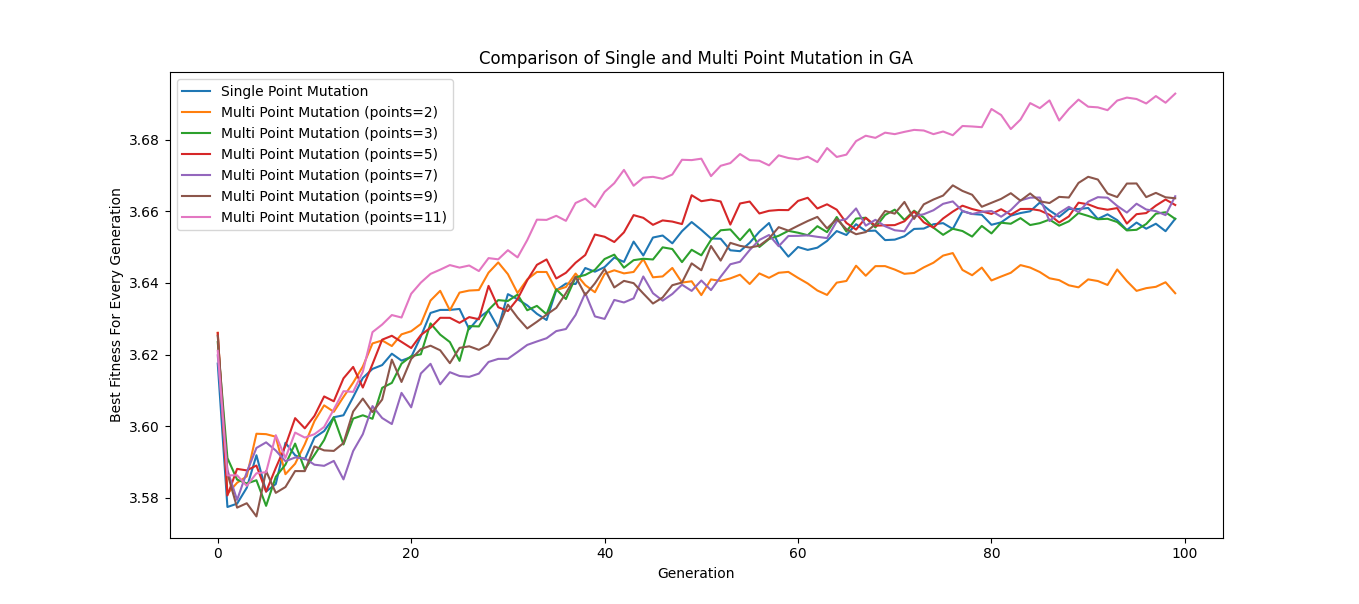
\includegraphics[width=0.95\textwidth]{../assets/img/ga_comparison_mutation.png}
  \caption{单点变异与多点变异的比较}\label{fig:}
\end{figure}

\subsection{结论}

多点变异的效果并不总是优于单点变异,具体效果需要根据问题的特性来选择变异方式。某些问题中,多点变异可能会导致过多的基因突变,从而影响收敛速度。因此,在实际应用中,应该根据具体问题的需要来选择适合的变异策略。

\section{Conclusion}

\subsection{文章总结}

本文对遗传算法中的欺骗问题进行了系统分析,尤其是在最小欺骗问题(MDP)框架下的表现。研究发现,遗传算法在面对欺骗性环境时,容易被引导到局部最优解,尤其在存在竞争模式的情况下,适应度较低的局部最优解可能会压倒全局最优解。因此,提升遗传算法的全局搜索能力、减少早熟收敛的风险成为关键改进方向。

为此,我们引入了无义密码子和动态变异率机制,成功提高了种群多样性,避免了算法过早收敛,并加速了全局最优解的搜索过程。无义密码子的引入增加了算法的自由度,减少了对初始参数设置的依赖,从而增强了算法的鲁棒性。而动态变异率机制则根据算法的运行状态自动调整变异强度,使得算法在早期阶段能够充分探索解空间,在后期阶段通过降低变异率加速收敛。

实验结果表明,结合动态变异率和多点变异策略的改进算法在解决复杂优化问题时,相较于传统的单点变异和固定变异率算法,展现了更强的全局搜索能力和更快的收敛速度。未来的研究可进一步探讨如何在更高维度的复杂问题中优化这些策略,尤其是在保证全局搜索能力的同时,进一步提高算法的收敛速度。

\subsection{感悟}

不要想当然:在设计算法时,往往认为某个优化策略实施后能有效解决之前的问题,因此期望实践中会表现得更好。然而,这往往忽视了新的策略可能带来的其他问题。有时,当理论分析遇到困难时,可以通过实验先行验证。而当实验结果不支持理论时,除了怀疑理论本身的正确性,也应考虑是否有其他限制条件导致了不良的结果。

\begin{Backmatter}

\bibliography{reference}
%\printbibliography

\end{Backmatter}

\end{document}
